\documentclass[11pt]{article}

\usepackage[a4paper,margin=2.6cm]{geometry}
\usepackage[T1]{fontenc}
\usepackage[utf8]{inputenc}
\usepackage{graphicx}
\usepackage{booktabs}
\usepackage{tabularx}
\usepackage{natbib}
\usepackage[hyphens]{url}
\usepackage{caption}
\usepackage[hidelinks]{hyperref}

\captionsetup{font=small,labelfont=bf}
\newcolumntype{L}{>{\raggedright\arraybackslash}X}
\newcommand{\pending}[1]{\textit{[Pending: #1]}}
\newcommand{\sqm}{m\(^2\)}

\title{Isobenefit Urbanism on real terrain: an open-source QGIS plugin
for simulating and planning walkable growth}

\author{%
Gareth Simons\thanks{Bartlett School of Planning, University College
London.} \and Tommaso Gabrieli\thanks{Bartlett School of Planning,
University College London. \pending{confirm the corresponding author.}}}

\date{}

\begin{document}

\maketitle

\begin{abstract}
\noindent
Isobenefit Urbanism proposes settlements in which every resident lives within
a walk of a mixed-use centre and of open green land. The published model
formalises this as a cellular automaton growing on a uniform abstract
plain. Building on that model, an open-source implementation carries the
rules onto real terrain, where existing towns, fragmented green space,
rivers, railways, motorways, and steep slopes shape what can be built. The
implementation turns the simulation into scenario sketches that prompt
discussion and feedback at the early stages of planning, ahead of
expert review and development. Its inputs come from
OpenStreetMap and the Copernicus GLO-30 elevation model, and distances
are bounded grid walks that detour around land unsuitable for building.
Existing fabric is frozen and served by its own centres, so the population
target counts new residents only. The pipeline runs a fifty-run
ensemble, scores every run on walkable access to centres and green, and
derives four outputs from the best single run: the raw grown state and
three plan options that share identical fabric and density, differ only
in centre arrangement, and keep every new home within the centre walk.
Three cases, each dominated by a different constraint, demonstrate the
pipeline: a new settlement at Cambourne, a green-belt release at Crews
Hill in London, and a hillside expansion at Pajarito in Medell\'in. A
fourth case removes the Rieselfeld and Vauban districts from Freiburg and
regrows the window toward their real population under two readings of
available land. The outcome ranges from regrowth almost wholly inside
the district boundaries to almost no growth, so the outputs depend
strongly on which land counts as available. All scenario data, parameters, and code are public, and the
results rebuild from committed sources at fixed seeds.
\end{abstract}

\section{Introduction}

Isobenefit Urbanism \citep{dacci2019} proposes that the benefits of a
settlement should be distributed evenly, as implied by the prefix
\emph{iso}, which means equal. Regardless of where one lives, a local
centre with shops, services, and workplaces, and open green land, are
both within a walk. The idea originates
in scenario work on isobenefit cities \citep{dacci2013}, and D'Acci later
formalised it as a cellular-automaton morphogenesis, which was published
with a Python simulator \citep{dacci_voto2023, voto_code}. The automaton
grows a grid of land cells under a small set of rules from seeded
centralities (the published model's term for centres),
and the walkability guarantee holds at every step however large the
settlement becomes. The approach sits between master-planning and
laissez-faire growth, because a few simple rules guide development while
the detailed form emerges \citep{dacci_banister_white2024}. As with
UrbanSim, an open model of land use and transport that entered use with
metropolitan planning agencies \citep{waddell2002}, an open simulation
tool can become a useful planning instrument. By incorporating
real-world constraints, we aim to make the isobenefit model similarly
useful for the early stages of the planning process.

The published model runs on an abstract grid, in which every cell
starts as nature, distances are straight lines, and a single radius, typically set to an
approximately fifteen-minute walk, governs access both to
centres and to green. This abstraction keeps the morphology of the
rules easy to study. In real-world use the model meets existing towns,
fragmented green space, rivers, railways, motorways, and steep slopes,
and its stochastic runs must become a drawing a planner can work with.
We therefore add the inputs, the constraints, and the post-processing
that carry the rules into this setting.

The contributions are:

\begin{enumerate}
\item An adaptation of the published rules to real geography. Existing
  fabric is frozen, so the model keeps built-up areas as they stand and
  focuses growth on open land. Designated green space is protected from
  development. Major roads, railways, and rivers become barriers
  that walking routes must detour around, slopes above a limit are
  treated as unsuitable for building, and distances are bounded grid
  walks, walking routes
  traced across the grid around these obstacles, in place of straight
  lines. Every departure from the published model is tabulated
  (Table~\ref{tab:rules}).
\item An open, reproducible implementation: a QGIS plugin that wraps a
  simulation engine published on PyPI, and accompanying documentation
  with explanatory material and worked scenarios.
\item A plan-derivation pipeline on top of the automaton. The
  likelihood layers blend an ensemble of runs and record how often each
  cell ends built, separating robust development locations from
  contingent ones. The plan options come from the best single run,
  judged on the lowest mean walk to centres and green. An optional
  post-processing refinement step improves the placement and
  arrangement of centres to consolidate access and arranges the highest
  densities around them, while the walk constraint is retained.
\end{enumerate}

The likelihood layers and the plan options are sketches for the early
stages of planning. They let a planner explore walkable
growth that retains the isobenefit principle, and they give residents
and other experts something concrete to discuss. We
demonstrate the pipeline on three case studies, each dominated by a
different constraint, and on a comparative case study that regrows two
well-studied walkable districts in Freiburg to show how the stochastic
outputs should be read against a realised outcome.
Sections~\ref{sec:background} to~\ref{sec:discussion} cover the background,
the methods, the case studies, the Freiburg comparison, and the
discussion.

\section{Background}
\label{sec:background}

\subsection{The published model}

The Isobenefit-cities simulator \citep{dacci_voto2023} grows settlements on a
square grid in which every cell starts as nature. Each simulation step scans
the grid against a frozen copy. A nature cell adjacent to built land is
eligible to become built on two conditions: the location must remain
within walkable reach of a centrality, the radius T\(^*\), typically
set to about one kilometre or a fifteen-minute walk, and building the
cell must not impinge on the green-space rules. Those rules
keep nature as one continuously connected region with a minimum
width of T\(^*\), so at no point does green space between built areas
narrow to below the walkable radius. An eligible cell builds by a random draw at each
step, so the built edge advances irregularly. If the build probability
is set to 0.5, for example, a cell has an even chance of building at
each step. New
centralities seed by rarer draws, either beside built land that has
outgrown its centres or on open land, and each built block draws its
population density from one of three tiers. The run stops at a
population cap. These rates, the tiers, and the cap are settings in
this implementation (Section~\ref{sec:rules}).

The automaton belongs to a long line of cellular models of urban form
\citep{white_engelen1993, batty2005, sante2010}. Unlike models fitted to observed
growth, its rules enforce a walkability guarantee while growth proceeds.

\subsection{Walking distances and standards}

We replace the single radius with two walking distances, one to a
centre and one to green space. Both are set in the QGIS plugin, whose
starting defaults of 800~m for the centre walk and 400~m for the green
walk are approximately ten-minute and five-minute walks respectively.
The walkable-city literature generally treats
destinations within a ten-to-fifteen-minute walk as walkable
\citep{moreno2021, abbiasov2024}, and observed walking distances for
everyday errands are of the same order \citep{yang_diezroux2012}. For
green space, the WHO Regional Office for Europe advises everyday access
within about 300~m straight-line distance \citep{who2016}, and Natural
England's accessible natural greenspace standard uses the same figure
\citep{naturalengland2010}. The 400~m starting default is slightly
longer than the advised 300~m because a walking route goes around
obstacles and covers more distance than the straight line.
Section~\ref{sec:cases} sweeps the centre walk across 400, 800, and
1{,}600~m, and the green walk stays at 400~m in the reported runs.

\section{Methods}
\label{sec:methods}

The QGIS plugin comprises two tools, one for data preparation and one
for simulation. The preparation tool downloads a scenario's input
layers from OpenStreetMap. This step is optional, because equivalent
layers can instead be supplied from the user's own data. Alternatively,
the user can download the layers and then edit them to reflect
different parameters or constraints. The simulation tool passes these inputs to the
engine, published on PyPI, which applies the growth rules and the
post-processing.

A scenario runs in a fixed sequence. The input layers set where growth
may occur, and the simulation tool rasterises them to a working grid.
The automaton then grows the settlement cell by cell: an empty cell
beside built land may build when a centre lies within the centre walk
and building would not break the green-space rules, and new centres
seed as the settlement outgrows its existing ones. An ensemble of runs
is blended into the likelihood layers, and the best single run is kept,
judged on walkable access. Post-processing then derives the plan
options from that run. The subsections below describe each of these
steps in turn.

\subsection{Real inputs}
\label{sec:inputs}

Each scenario is defined by a simulation boundary in a metric coordinate
reference system and a set of vector layers. The worked scenarios fetch
these layers from OpenStreetMap
\citep{osm} with the preparation tool. The layers cover existing
built fabric, green space to preserve, existing mixed-use centres,
unbuildable land (the areas treated as unavailable for development),
streets, public-transport stops, rail and tram stations,
railways, and industrial land. Terrain slope bands at 15, 20, 25, and 30
degrees are derived from the Copernicus GLO-30 elevation model
\citep{copernicus_glo30} and ship as a separate editable layer, so users
can trim or extend them from local knowledge before the selected bands
join the unbuildable layer.

\subsection{Grid preparation}
\label{sec:gridprep}

The simulation tool prepares the grid before growth begins. It
rasterises the input layers to a working grid at a user-selected cell
size, typically up to 50~m, though it may be preferable to work at a
higher resolution. Existing built fabric is frozen, meaning
the simulation leaves it unchanged. Corridors are carved from motorways,
trunk roads, railways, and rivers and marked unbuildable, so the
bounded grid walk detours around them and development cannot extend
across them. The remaining street geometry stays on the map as context
only.

Preparation also separates developable land from land that cannot
carry development. Developable land must be locally wide, spanning a
three-by-three block of open cells or lying immediately beside one,
and it must belong to a contiguous wide region large enough to hold
the minimum settlement, where contiguity counts shared edges only.
Land that fails either test is reclassified as protected green: it
stays walkable and counts as green space, and a sliver between
buildings or an enclave inside a town reads as a pocket park. Growth,
seeding, and centre provision are never spent on it, so doomed
satellites and piecemeal infill of scraps are ruled out before the
run.

Freezing also separates existing development from new. The input data
rarely support a rigorous estimate of the existing population or its
distribution, so the model treats existing residents as served by
their existing centres and counts only new residents toward the
population target. A given target therefore represents the same amount
of new development in an empty study window and in one that contains
an existing town.

Growth and scoring share one distance metric, the bounded grid walk,
which is blocked by unbuildable land and computed with a Dijkstra
search bounded at the maximum walking distance. Street-network distances
were tested in earlier releases and removed because the streets of a
new settlement do not yet exist, which forced a hybrid of network
distances over existing streets and assumed routes over new fabric
that was difficult to justify.

\subsection{The growth rules}
\label{sec:growth}

A run proceeds in iterations. Each iteration applies the growth rules
to every land cell, visiting the cells in a shuffled order to avoid the
directional bias of a fixed scan. A cell is a candidate for building
when it is empty, buildable, and touches built land, which keeps growth
attached to the existing fabric. A candidate must remain within
the centre walk of a centre, which keeps new homes within walkable
reach of shops and services. Building it must also leave the green network
intact: a green corridor between developments may not narrow below the
minimum green span, and a split must leave each fragment a minimum
contiguous area. A candidate that passes every check builds at the
configured build probability, which makes growth stochastic, staggers
the built edge, and sets the pace of growth. Each built cell draws one
of the three density tiers at the configured shares.

New centres arise in two ways. Where the settlement has outgrown its
centres, so that a cell at the growing edge would exceed the centre
walk to every existing and grown centre, that cell may itself become a
new centre and seed development around it. The conversion is again a
random draw at a configurable seeding probability, at most one new
centre per iteration, and seeding stops once the run reaches 80\% of
the population target. Separately, a dispersal probability allows
leapfrogging: an isolated centre may seed on open land by a per-cell
draw, at a rate the dispersal setting controls, and begin a new
satellite settlement around it. A run stops when it
reaches the population target.

\subsection{Ensembles and selection}
\label{sec:ensemble}

An ensemble comprises a configurable number of runs, which is fifty in
every scenario reported here. Each run starts from the same inputs,
draws its own seed, and grows into a complete settlement pattern that
satisfies the constraints. Because the draws differ, different runs
build in different places. The likelihood layers record, for each
cell, the fraction of runs in which it ended built or green. A cell
built in most runs is a robust development location, and a cell built
in only a few is contingent.

Each run satisfies the constraints, but a blend of many runs can
violate them, because the runs disagree cell by cell. One run keeps a
cell open as part of a green corridor while another builds on it, so
the layers record an intermediate fraction there, and a map assembled
from the most frequently built cells follows the corridor routing of
no single run. The layers therefore show where development is likely,
and we do not read the plan off them. Instead, we post-process every
run in the same way into a candidate plan
(Section~\ref{sec:fouroutputs}) and select the one with the lowest
mean walk to a centre and to green.

We also
report served coverage, the share of homes within the chosen walks of
both a centre and a qualifying park. A contiguous green patch
qualifies as a park when its area reaches the square of the minimum
green span, which is 16 hectares at the 400~m default. Both measures
use the bounded grid walk of the growth rules, judging the centre and
the green distance each against its own walk, and a reported mean walk
averages over the homes within that walk of the amenity.

\subsection{Post-processing and the four outputs}
\label{sec:fouroutputs}

A finished run leaves the raw grown state, and everything that follows
is post-processing on that state. A stochastic run can still leave
stranded fragments, detached clusters of new growth that stayed below
the minimum settlement size. Post-processing therefore applies two
steps before the centre options: pruning of these fragments and a
density arrangement.

Pruning reverts a detached sub-threshold cluster to nature, because it
is not viable development. An outlying hamlet receives the same
judgment: where a settlement of existing fabric is itself below the
minimum size and has no centre of its own, its new growth reverts,
while the existing buildings stay. A cluster grown against a centred
town is kept whatever its size, because its growth was anchored on
that town's centres and counts as legitimate infill. Existing fabric
is never pruned, and pruning is the only step that changes the
population, so a plan option can carry less than the raw state.

Density arrangement then revisits the tiers the run drew. Each new
home was built at one of the three density tiers at the configured
shares, and post-processing moves the drawn values spatially so the
highest tiers sit nearest the final centres. The shares, and therefore
the population, are fixed by the run.

Four outputs are then written. The \emph{raw} output shows the best single
run exactly as it grew before any post-processing and colours each cell by
the density tier the run drew there; the best single run is rerun at its
own seed to recover this drawn density grid. The three plan options share
identical built fabric and identical
arranged density and differ only in centres. \emph{As grown} keeps every
centre exactly where the run seeded it. \emph{Optimised placement}
repositions each centre central to the homes it serves and adds one
wherever new development lacks provision within the walk; existing
centres serve the existing fabric and any sub-threshold infill within
their walk, so a scrap of infill does not receive a centre of its own. \emph{Fewest centres} additionally
removes centres one at a time for as long as every home keeps one within
the walk.

Every option enforces the same constraint: no edit may leave a new
home beyond the centre walk of a centre. A repositioning or removal that would strand a
home is discarded, and gap-filling additions are never blocked. Each centre
is sized by the population in its catchment, existing centres and rail
or tram station anchors stay fixed, and every settlement with new
development keeps at least one attached centre. The raw state is
written alongside the options and the run report records coverage for
all four outputs, so every edit the post-processing made stays visible
and comparable. Optimised placement is the recommended plan, so run
selection scores each run's optimised-placement candidate, and the case
studies and the Freiburg comparison below report that option.

\subsection{Public transport}
\label{sec:transit}

Rail and tram stations join the automaton's centre seeds, so development
gathers around them. In post-processing they are treated as fixed anchors
(Section~\ref{sec:fouroutputs}) and sized like any other centre. All stops
and stations feed reported transit metrics (coverage, access, and mean
walk), which inform the reader without influencing run selection. Density
arrangement reinforces this access, because a stop beside a well-placed
mixed-use centre surrounded by the densest tiers serves the most people
and destinations.

\subsection{Rule adaptations}
\label{sec:rules}

In summary, Table~\ref{tab:rules} records the treatment of each
published rule
under four statuses: unchanged, reparameterised (same rule, different
units or defaults), modified (behaviour differs), or extension (no
counterpart in the published model). Most of the modifications extend the published model
from its uniform abstract plain to the real inputs of
Section~\ref{sec:inputs}.

\begin{table}[p]
\centering
\caption{The published rules \citep{dacci2019, dacci_voto2023, voto_code}
and their treatment in this implementation.}
\label{tab:rules}
\small
\begin{tabularx}{\textwidth}{L L l}
\toprule
Published rule & This implementation & Status \\
\midrule
Build only on nature cells adjacent to built land &
Same: a candidate must be empty and touch built land &
Unchanged \\
\addlinespace
A centrality must lie within T\(^*\) of the new cell, straight-line &
A centre must lie within the centre walk, a bounded walk over the grid that
cannot cross unbuildable land &
Modified \\
\addlinespace
Build with probability 0.5 once checks pass &
Same mechanism; default 0.25 &
Reparam. \\
\addlinespace
Nature continuously connected, with a minimum width of T\(^*\) &
Local rules: no green corridor between developments may pinch below the
minimum span (strips bounded by water or a carved corridor exempt), and a
split must leave each fragment a minimum contiguous area &
Modified \\
\addlinespace
Every built cell keeps nature within T\(^*\) &
Same, as a bounded walk; the check also covers the newly built cell &
Unchanged \\
\addlinespace
New centralities seed near under-served built land, probability 0.005 &
Same trigger at probability 0.01; at most one new centre per iteration;
seeding stops at 80\% of the population target &
Modified \\
\addlinespace
Isolated centralities seed on open land, probability 0.1 scaled by area &
Per-cell probability without area scaling, exposed as off, moderate, or
aggressive dispersal &
Reparam. \\
\addlinespace
One radius T\(^*\approx1\)~km &
Explicit metres; two distances, default 800~m to a centre and 400~m to green &
Reparam. \\
\addlinespace
Density drawn from three tiers at probabilities 0.7 / 0.3 / 0 &
Same draw with tiers and shares as settings; post-processing arranges the
drawn values so the highest tiers sit nearest the final centres &
Modified \\
\addlinespace
Run stops at a population cap &
Same stop; the target counts new residents only &
Modified \\
\addlinespace
Fixed raster scan order against a frozen grid copy &
Shuffled visit order each iteration, removing scan-direction bias &
Modified \\
\addlinespace
One run, one output &
Ensembles: many runs blended into likelihood layers; best single run
selected &
Extension \\
\addlinespace
Grid starts as uniform nature &
Real OpenStreetMap inputs: frozen built fabric, protected green, carved
barriers, centres, stops, and stations &
Extension \\
\addlinespace
All nature is available to build &
Developable land must be locally wide and belong to an edge-connected
wide region able to hold the minimum settlement; all other open land
is reclassified as protected green before the run &
Extension \\
\addlinespace
Centralities stay where seeded &
Three centre options in post-processing, all keeping every home within the
centre walk &
Extension \\
\bottomrule
\end{tabularx}
\end{table}

\subsection{Software and reproducibility}
\label{sec:software}

The implementation comprises a simulation engine and a QGIS plugin. The
simulation engine is a Rust crate, published on PyPI as
\texttt{isobenefit}, which exposes a small arrays-in-arrays-out API
through PyO3 and never imports QGIS. The QGIS
plugin \citep{qgis} supplies data preparation, the run dialog, and the
post-processing and reporting layer, and depends only on what QGIS already
bundles plus the engine. The QGIS plugin repository does not permit
shipping binaries, so the compiled engine installs from PyPI and the
plugin offers to install it on first run.

Results are deterministic and independent of thread count. Every stochastic
draw derives from a per-work-item seed, and parallel reductions are
order-independent integer sums. Cross-checks between the Rust engine and a
reference Python implementation of the walk metric and component labelling
run in the test suite. A single verification script runs the full gate
(formatting, linting, Rust and Python tests, and the website build) and mirrors CI
exactly; releases are tagged, version-locked between engine and plugin, and
published automatically. All scenario inputs are committed, so every result
in this paper rebuilds offline from source at fixed seeds.

\section{Case studies}
\label{sec:cases}

We ran the pipeline on three demonstration cases, in each of which a
different constraint dominates the outcome: a
free-standing new settlement (Cambourne, UK), a green-belt release at a
metropolitan edge (Crews Hill, London), and a topography-bound hillside
expansion (Pajarito, Medell\'in). Four further scenarios (Dnipro, Celina,
Kigali East, and the Freiburg comparison of Section~\ref{sec:freiburg})
ship in the repository with the same file anatomy. Table~\ref{tab:scenarios}
gives the settings; we translated local density norms into the model's
three-tier control.

The cases are hypothetical demonstrations, and none reflects a
real-world development priority or a proposal for the place it depicts.
The windows, the targets, and the density presets are our demonstration
settings, chosen to exercise the constraints. An application in practice
would set them in dialogue with residents, planners, and local experts,
who hold the knowledge of ownership, commitments, and local intent that
stays outside the inputs.

All metrics below come from full-resolution runs of the committed
scenarios (fifty-run ensembles at the grids of Table~\ref{tab:scenarios},
seed 42), which \path{scripts/paper_metrics.py} regenerates.

\begin{table}[t]
\centering
\caption{Case-study settings. Tiers are people per km\(^2\) (high / medium /
low) with shares in the same order; all cases use an 800~m centre walk,
400~m green walk, a 1{,}000-person minimum settlement, 400~m minimum green
span, and fifty ensemble runs.}
\label{tab:scenarios}
\small
\begin{tabularx}{\textwidth}{l L L L}
\toprule
 & Cambourne & Crews Hill & Pajarito \\
\midrule
Theme & New settlement & Green-belt release & Hillside expansion \\
CRS / grid & EPSG:27700, 50~m & EPSG:27700, 25~m & EPSG:32618, 25~m \\
Target (new residents) & 30{,}000 & 13{,}000 & 40{,}000 \\
Tiers & 6{,}000 / 3{,}000 / 1{,}500 & 26{,}000 / 15{,}500 / 9{,}500 &
35{,}000 / 18{,}000 / 8{,}000 \\
Shares & 0.2 / 0.3 / 0.5 & 0.2 / 0.5 / 0.3 & 0.3 / 0.4 / 0.3 \\
Dispersal & Moderate & Off & Moderate \\
Slope limit & None & None & Over 20\(^\circ\) unbuildable \\
\bottomrule
\end{tabularx}
\end{table}

\subsection{Cambourne: a new settlement and the four outputs}

Cambourne, a fast-growing Cambridgeshire new settlement, is the reference
case. The 30{,}000 target is hypothetical and reflects no assessment of
local housing need. Figure~\ref{fig:cambourne} shows the study window before growth and under
three centre-walk settings. At the baseline 800~m walk, the plan
accommodates about 13{,}600 of the 30{,}000 target with 86\% of all homes
served (within the walk of both a centre and green), a mean centre walk
of 295~m, and a mean green walk of 94~m. The window's developable land,
after the availability rule sets aside what cannot carry a settlement,
does not hold the full target at the baseline settings.

Table~\ref{tab:fouroutputs} reproduces the run report for a smaller
12{,}000-person Cambourne window used as the worked demonstration of the
four outputs, which \path{scripts/demo_run_report.py} regenerates. The raw grown state credits 84\% of the target, and pruning reduces
this to 62\%. This window grows part of its population as detached
satellite clusters that stay below the 1{,}000-person minimum, and
pruning reverts them to nature. Served coverage holds at 93--97\%
across all four outputs. Among the three plan options, which differ
only in centres, optimised placement cuts the mean centre walk from 259
to 235~m with one more centre area than as grown (19 against 18), and
fewest centres removes two of those centre areas at the cost of most
of the reduction (255~m). Fewest centres starts from the optimised
placement and removes centres only while every home keeps one within
the walk.

\begin{table}[t]
\centering
\caption{Run report for the Cambourne demonstration window (12{,}000-person
target): the raw grown state and the three plan options.}
\label{tab:fouroutputs}
\small
\begin{tabular}{l r r r r}
\toprule
Metric & Raw & As grown & Optimised placement & Fewest centres \\
\midrule
Population accommodated & 10{,}132 & 7{,}410 & 7{,}396 & 7{,}396 \\
Share of target & 84\% & 62\% & 62\% & 62\% \\
Built cells (incl.\ existing) & 2{,}075 & 1{,}691 & 1{,}691 & 1{,}691 \\
Mixed-use centre areas & 25 & 18 & 19 & 17 \\
Served coverage (centre and green) & 97\% & 93\% & 93\% & 93\% \\
Mean walk to a centre (m) & 291 & 259 & 235 & 255 \\
Mean walk to green (m) & 113 & 114 & 114 & 114 \\
Centre \sqm{} per person & 4 & 19 & 19 & 19 \\
Green \sqm{} per person & 674 & 1{,}051 & 1{,}053 & 1{,}053 \\
\bottomrule
\end{tabular}
\end{table}

\begin{figure}[p]
\centering
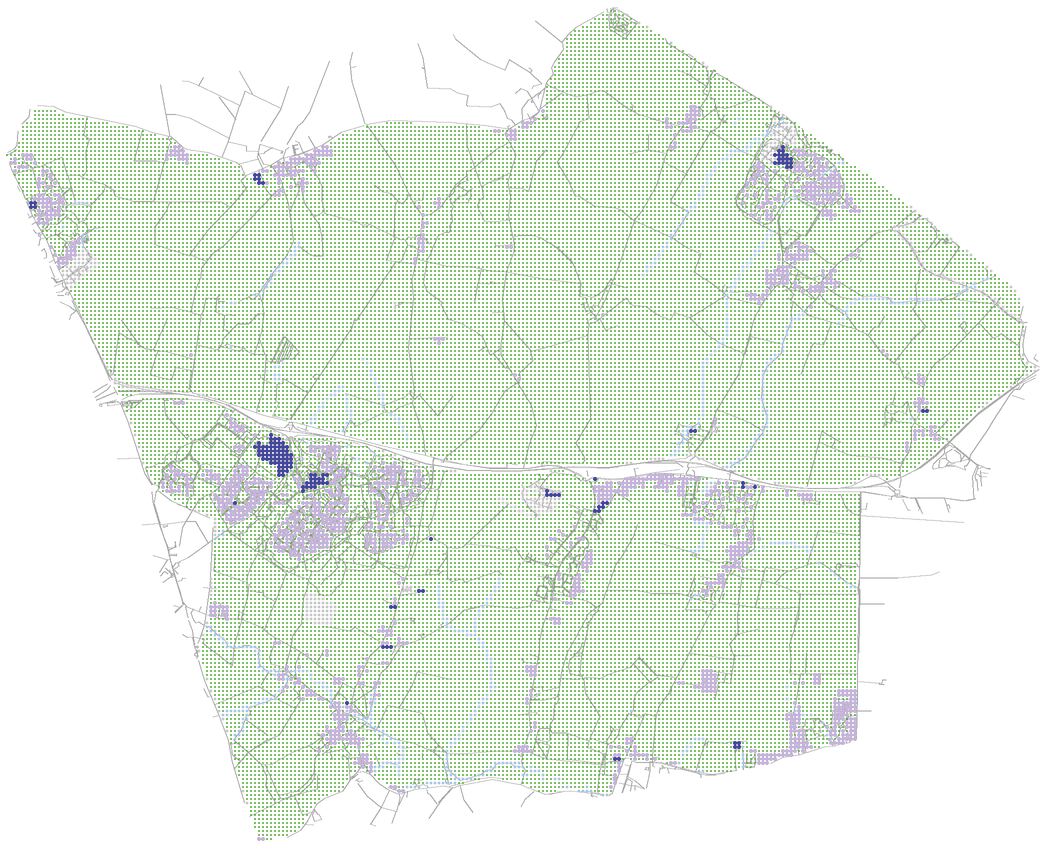
\includegraphics[width=0.48\textwidth]{figures/cambourne_existing.png}\hfill
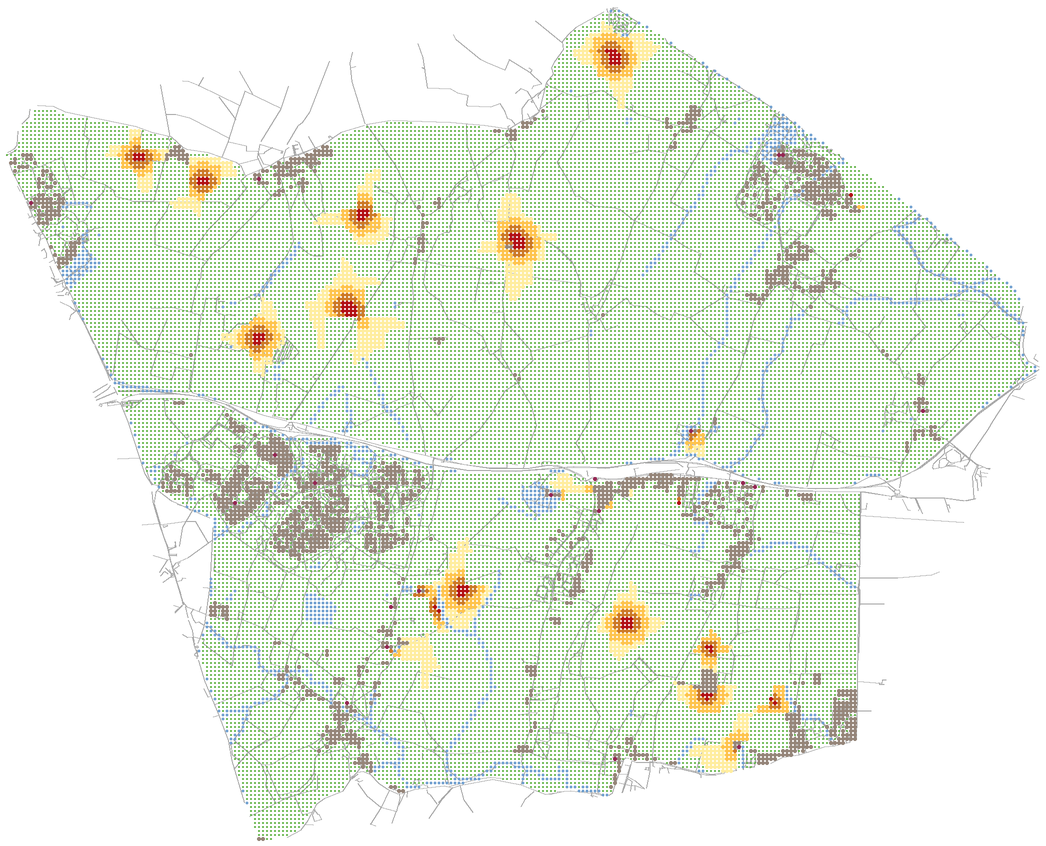
\includegraphics[width=0.48\textwidth]{figures/cambourne_baseline.png}\\[2pt]
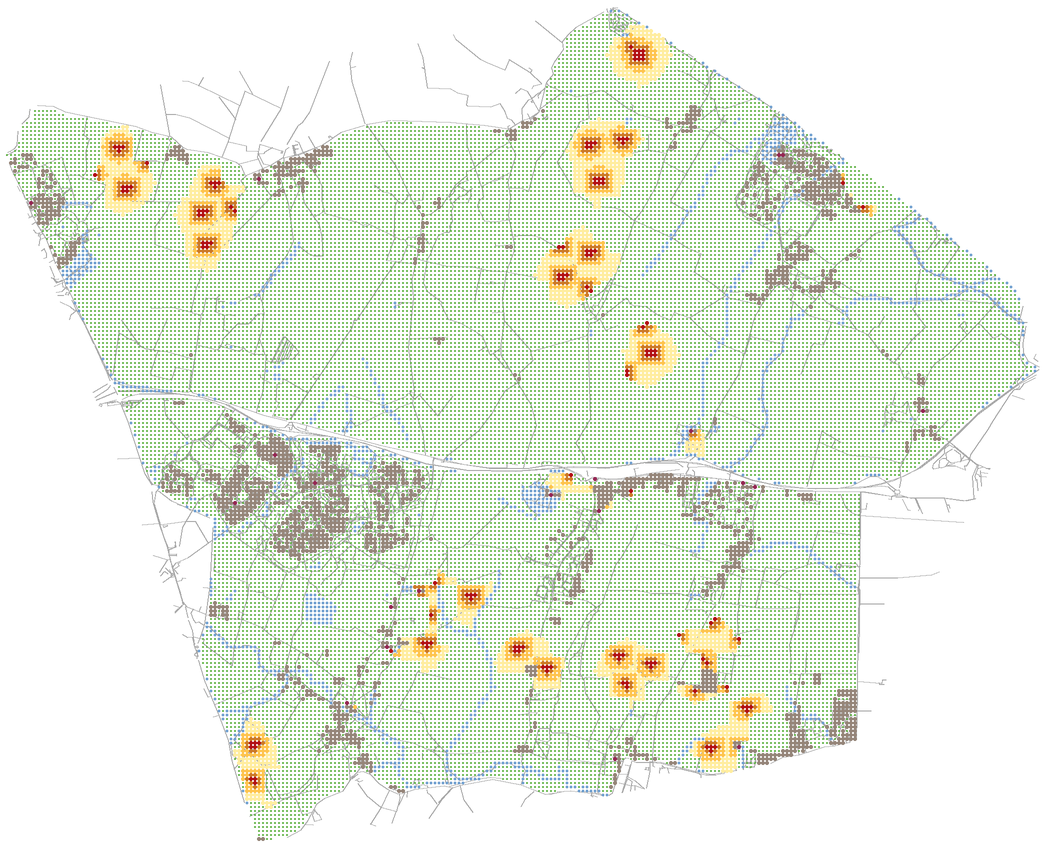
\includegraphics[width=0.48\textwidth]{figures/cambourne_walk400.png}\hfill
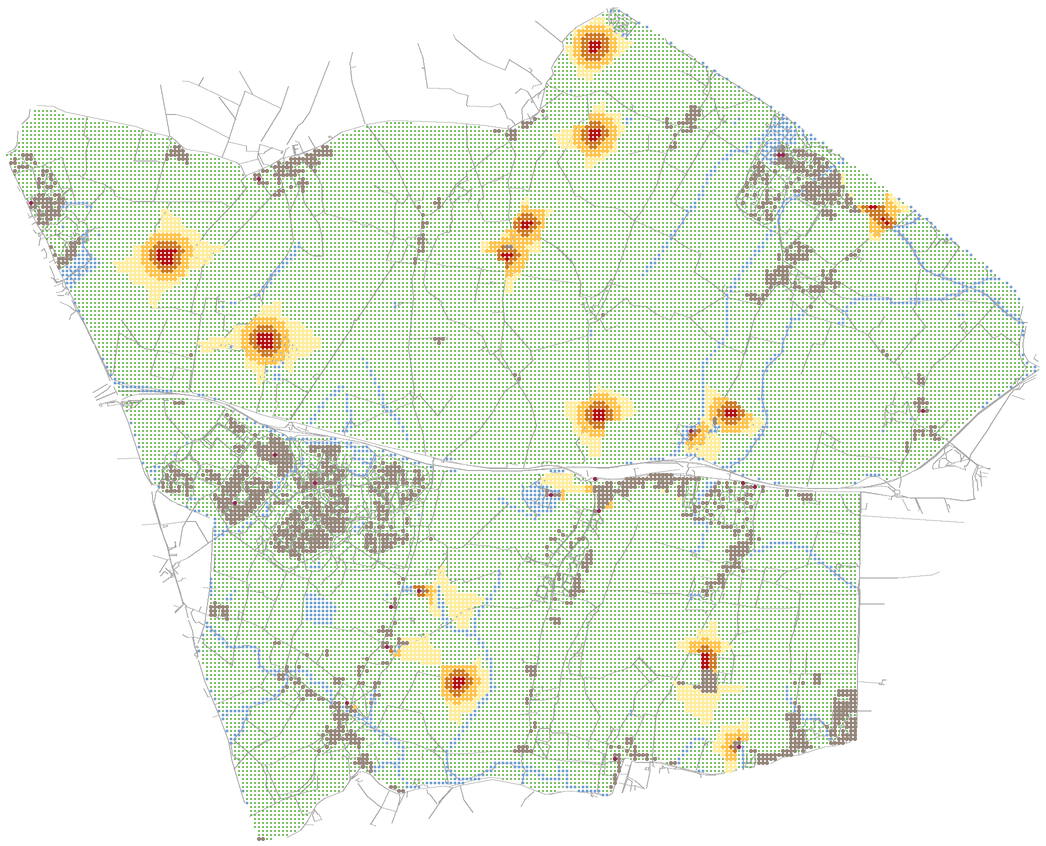
\includegraphics[width=0.48\textwidth]{figures/cambourne_walk1600.png}
\caption{The Cambourne window before growth (top left) and the
recommended plan at centre walks of 800~m (top right), 400~m (bottom
left), and 1{,}600~m (bottom right). Served coverage rises with the
permitted walk. Full scenario resolution, seed 42.}
\label{fig:cambourne}
\end{figure}

\subsection{Crews Hill: a green-belt release}

The Crews Hill area of Enfield, inside the M25 at London's northern edge,
is one of the largest green-belt releases proposed in an emerging London
local plan, which allocates about 5{,}500 homes around an existing rail
station. We built the scenario to test whether a release delivers a walkable
settlement or car-led sprawl, and which green network survives. Dispersal
is off, so the extension grows contiguously. The density tiers use
indicative UK design-code values (40 / 65 / 110 dwellings per hectare at a
household size of 2.36). The scenario takes from the emerging plan only
the site boundary and the allocation's scale, as a hypothetical reading
of the site. Whether the release should proceed is a question for the
plan's examination and its public consultation.

At the baseline walk the plan accommodates about 11{,}700 of the
13{,}000
target with 75\% of homes served, a mean centre walk of 271~m, and a mean
green walk of 106~m (Figure~\ref{fig:crewshill}). Shifting the shares
one step toward the high tier houses 7\% more people on 4\% fewer built
cells, so within the release boundary the denser preset saves land
without a population cost. The station anchor holds the main centre against the rail
line, so the walkable structure forms around the site's one existing
piece of transport infrastructure.

\begin{figure}[p]
\centering
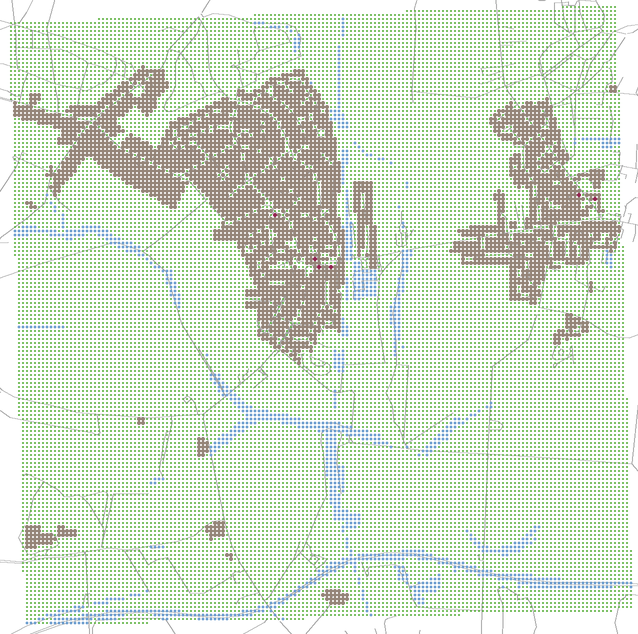
\includegraphics[width=0.48\textwidth]{figures/london_crews_hill_existing.png}\hfill
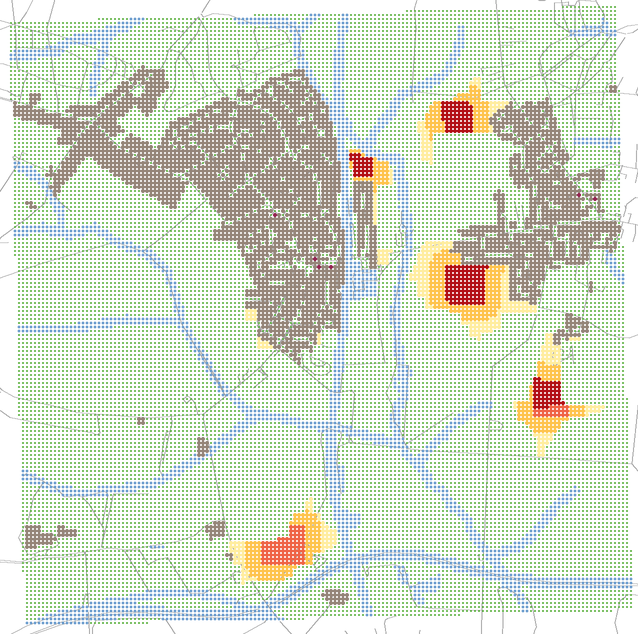
\includegraphics[width=0.48\textwidth]{figures/london_crews_hill_baseline.png}\\[2pt]
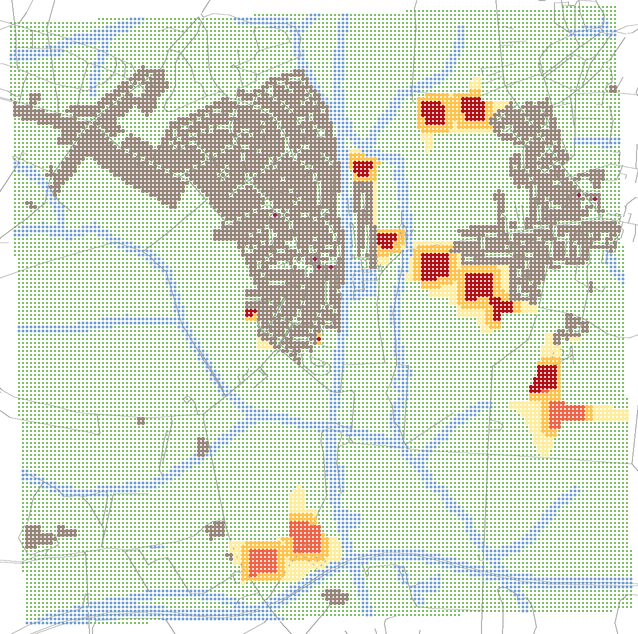
\includegraphics[width=0.48\textwidth]{figures/london_crews_hill_walk400.png}\hfill
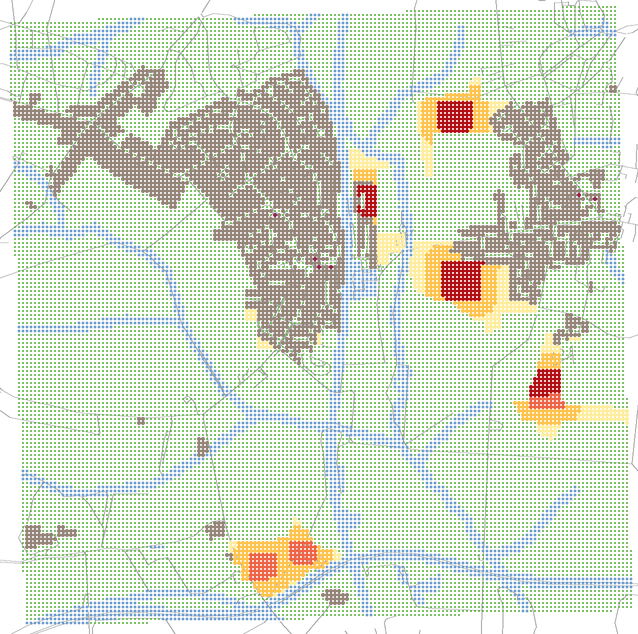
\includegraphics[width=0.48\textwidth]{figures/london_crews_hill_walk1600.png}
\caption{The Crews Hill window before growth (top left) and the
recommended plan, with dispersal off, at centre walks of 800~m (top
right), 400~m (bottom left), and 1{,}600~m (bottom right). The station
anchor holds the main centre against the rail line at every setting.
Full scenario resolution, seed 42.}
\label{fig:crewshill}
\end{figure}

\subsection{Pajarito, Medell\'in: topography as the dominant constraint}

Pajarito and Ciudadela Nuevo Occidente on Medell\'in's northwestern slopes
are a planned expansion of high-rise social housing served by the
Metrocable. Slopes over 20 degrees are unbuildable and cover about 30\% of
the study window, so the green network and the short walking distances
must fit around the terrain. The high density tier (35{,}000 people per
km\(^2\)) reflects the area's housing towers. The scenario is a
hypothetical exercise on the district's terrain and carries no
recommendation for its future development.

At the baseline walk the plan accommodates about 29{,}400 of the 40{,}000
target with 76\% of homes served and a mean centre walk of 221~m
(Figure~\ref{fig:medellin}), with the steep-slope mask fragmenting the
buildable land. The coverage figure counts the substantial existing hillside fabric
in the window as well as the new growth, so it reads low even where new
growth is well served. Turning dispersal off
lowers both the accommodated population (25{,}100) and coverage
(54\%), because contiguous growth cannot reach the buildable benches
that only satellite seeding can start.

\begin{figure}[p]
\centering
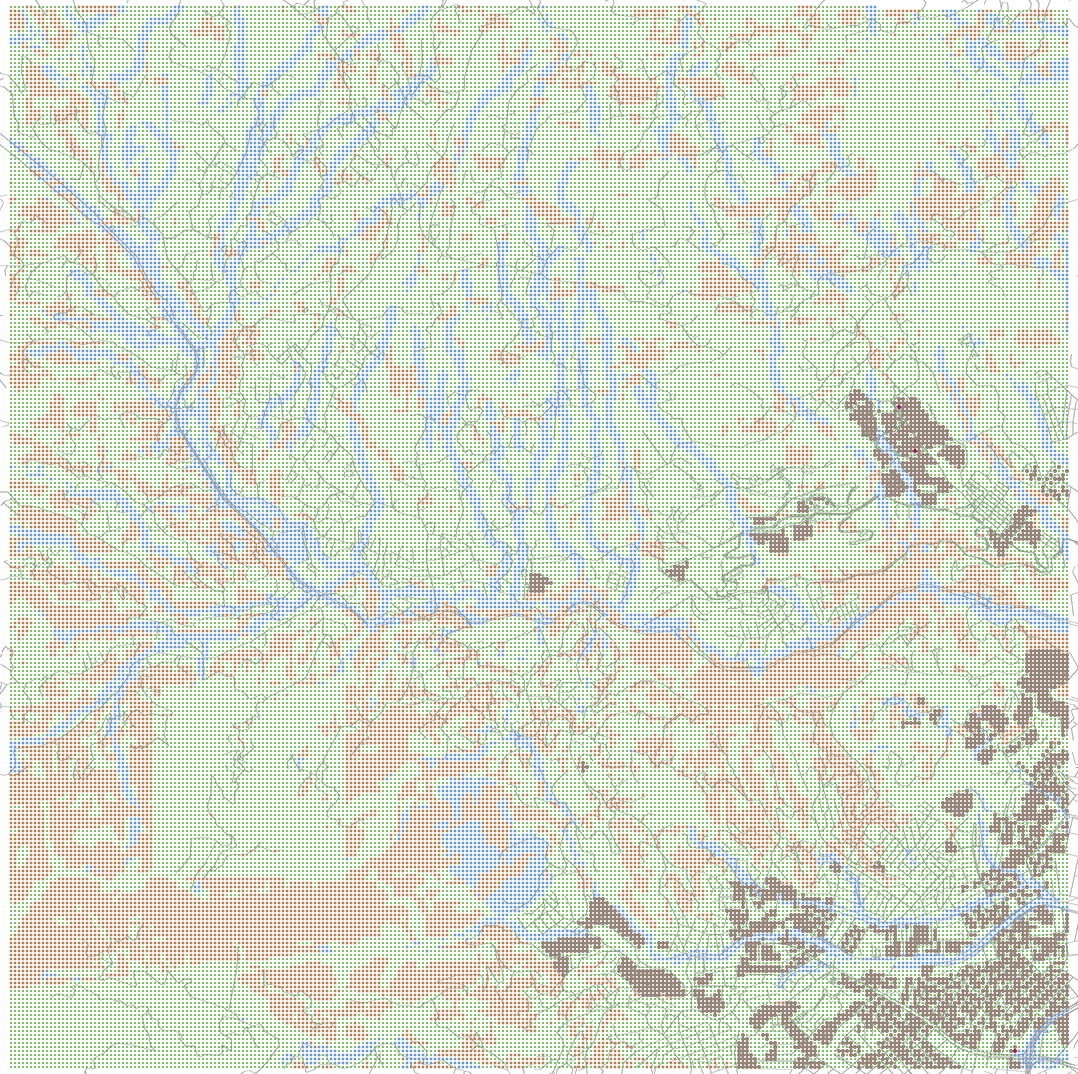
\includegraphics[width=0.48\textwidth]{figures/medellin_pajarito_existing.png}\hfill
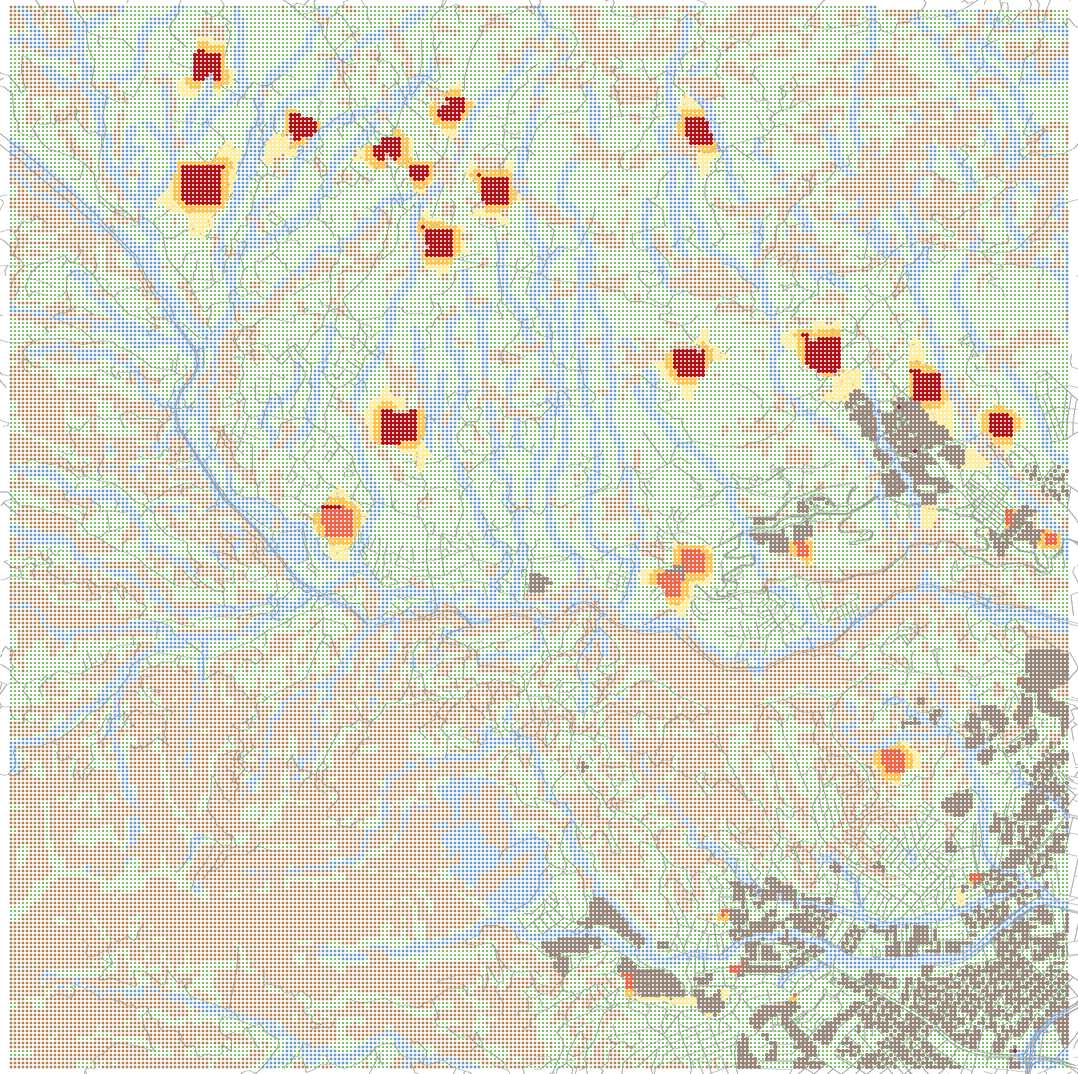
\includegraphics[width=0.48\textwidth]{figures/medellin_pajarito_baseline.png}\\[2pt]
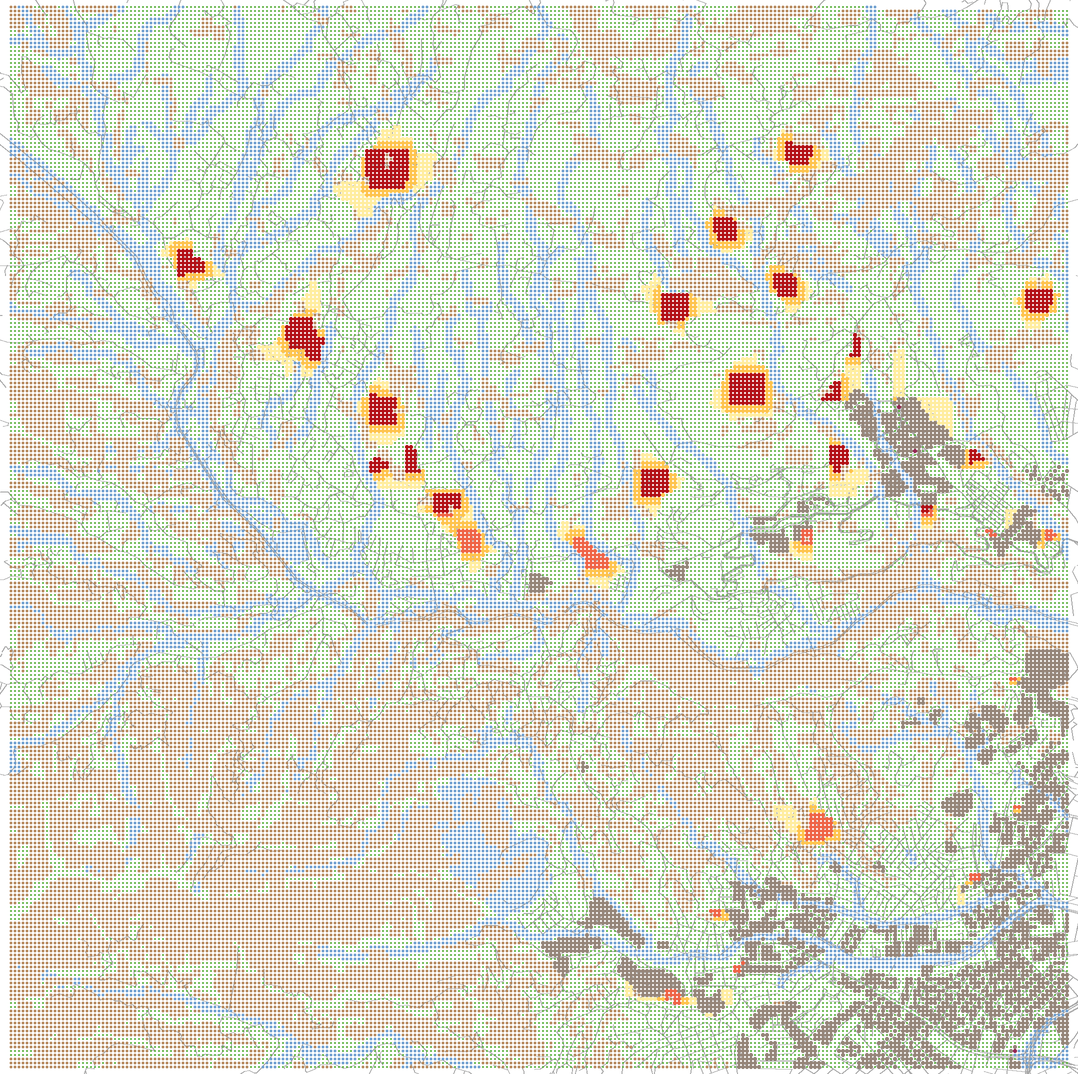
\includegraphics[width=0.48\textwidth]{figures/medellin_pajarito_walk400.png}\hfill
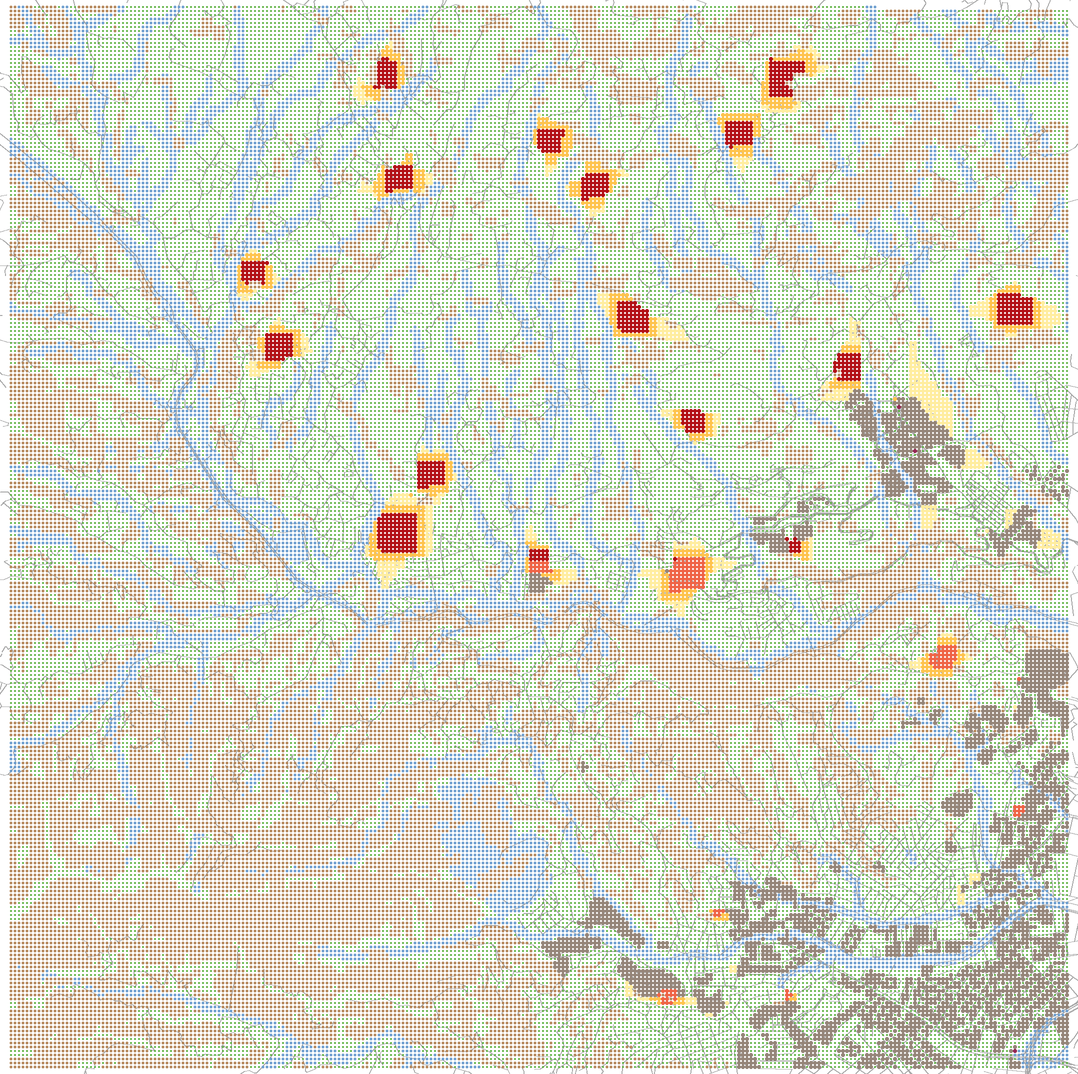
\includegraphics[width=0.48\textwidth]{figures/medellin_pajarito_walk1600.png}
\caption{The Pajarito window before growth (top left) and the recommended
plan at centre walks of 800~m (top right), 400~m (bottom left), and
1{,}600~m (bottom right). Slopes over 20\(^\circ\) are unbuildable and
fragment the buildable land. Full scenario resolution, seed 42.}
\label{fig:medellin}
\end{figure}

\subsection{Sensitivity to the centre walk}

Table~\ref{tab:sweep} sweeps the centre walk across 400, 800, and
1{,}600~m for the three cases. A longer permitted walk lengthens the
mean walk in every case and raises served coverage at Cambourne (74\%
to 99\%) and Crews Hill (61\% to 88\%). Pajarito moves least, and not
monotonically, because the terrain mask binds the form before the
centre walk does and each figure comes from one selected run. Windows
dominated by existing fabric sit lower on the coverage metric, which
counts every home in the window (Section~\ref{sec:discussion}).

\begin{table}[t]
\centering
\caption{Served coverage and mean centre walk under three centre-walk
settings. Coverage counts all homes in the window, including existing
fabric; the mean walk averages over homes within reach of a centre.}
\label{tab:sweep}
\small
\begin{tabular}{l rr rr rr}
\toprule
 & \multicolumn{2}{c}{400~m} & \multicolumn{2}{c}{800~m (baseline)} &
\multicolumn{2}{c}{1{,}600~m} \\
Scenario & Cov. & Walk & Cov. & Walk & Cov. & Walk \\
\midrule
Cambourne & 74\% & 163~m & 86\% & 295~m & 99\% & 433~m \\
Crews Hill & 61\% & 146~m & 75\% & 271~m & 88\% & 392~m \\
Pajarito & 63\% & 110~m & 76\% & 221~m & 72\% & 280~m \\
\bottomrule
\end{tabular}
\end{table}

\section{A comparative case study: regrowing Rieselfeld and Vauban}
\label{sec:freiburg}

Rieselfeld and Vauban in western Freiburg are two widely studied walkable
districts, which were planned in the 1990s and are often cited as models
of the form this tool aims for. We ran the model where a realised outcome
exists, to show how the outputs read against a known answer. A stochastic
workflow generates many valid outcomes, and the realised districts are one
of them. The exercise is retrospective, and we draw from it no
implication for Freiburg's planning. The two district boundaries, which are fetched from
OpenStreetMap and cached with the scenario, are removed from the built
input together with the one centre seed inside them. The model then regrows the window toward the
districts' real combined population of about 16{,}000, using the committed
scenario parameters at the full 25~m resolution with fifty runs: dispersal
off, tiers of 22{,}000 / 14{,}000 / 8{,}000 people per km\(^2\) at shares
0.2 / 0.6 / 0.2, and the default walks, minimum settlement, and green
span. We scored the optimised-placement output and the real districts on
the same metrics. Their built cells count as the development
under assessment, the OpenStreetMap-mapped centres in the window stay
active, and the centres inside the districts count as the districts' own.

The comparison is only meaningful if the real world and the simulation
start from the same availability of land. The scenario's built layer
derives from OpenStreetMap landuse polygons, and we audited an early run
(the scripts \path{check_freiburg_landclass.py} and
\path{check_freiburg_builtgap.py}) and found growth escaping to land
those polygons show as open, which on inspection was a hospital campus
and a cemetery. A
supplementary availability layer therefore closes the gap identically in
the simulation inputs and in the real-district scoring: hospital and
university campuses, railway land, and construction sites join the frozen
built fabric, and cemeteries join unbuildable land. The audit and the
patch preceded the concentration result reported below, so the patched
layer contributes to that result. Regional-plan set-asides may not
reach OpenStreetMap, so some open land may still be withheld in practice.

What counted as available land then admits two readings, and we ran
both. The pre-plan reading also removes the protected
green inside the boundaries, because the whole former sewage field was
open to the 1990s planners and the Freiburger Rieselfeld reserve beside
the built district was designated as compensation as part of its
development. The present-day reading keeps every committed green
designation intact. Table~\ref{tab:freiburg} and Figure~\ref{fig:freiburg}
report both.

Under the pre-plan reading, the model regrows 1{,}304 cells housing about
11{,}700 residents, and over 99\% of that growth falls inside the
district boundaries, nearly all of it in Rieselfeld. The containment
stops short of footprint agreement, because
the cell-level overlap with the real footprint is weak (intersection over
union 0.12) and the build likelihood sits higher on the land the
planners set aside for the reserve (0.18) than on the land they built
(0.14). The regrown plan's mean walks are shorter than the real
districts' (368~m against 397~m to a centre), which follows from the
construction: the scored output is optimised placement, whose objective
minimises the mean centre walk under the 800~m cap, and run selection
keeps the lowest-mean-walk run.

The containment follows from the availability rule and two growth
rules. The availability rule leaves the Rieselfeld field as the one
large developable region near the removed districts, while the
scattered growable land elsewhere in the window fails the width or
capacity test and is set aside. Growth must then touch existing fabric
and keep a centre within the 800~m walk, and at the start only a
handful of the field's cells lie within the walk of the one existing
centre on its eastern edge, so every
run enters the field where the real district also attaches to
the town. Vauban's open strip fares differently: it is narrower than
the minimum width over most of its length, so the availability rule
sets nearly all of it aside as protected green, and the two or three
cells that remain grow and stop. The real Vauban sits outside what the
availability and growth rules permit at their defaults, at every green
span in the sweep.

We varied the minimum green span, which is the rule that binds here,
across 200, 400, and 600~m (Table~\ref{tab:span}). Footprint
agreement with the real districts falls as the span grows, from an
intersection over union of 0.15 at 200~m to 0.08 at 600~m. The real
districts also score lower on the model's own served coverage as the span
grows, because fewer of their internal parks qualify (54\% at 200~m
against 37\% at 600~m). The 49\% score at the default span reads the same
way, since park qualification scales with the span
(Section~\ref{sec:ensemble}) and served coverage is a threshold score.
Both movements indicate that
Rieselfeld and Vauban were built at a green grain finer than the model's
default 400~m. Vauban's regrowth stays at two or three cells across
the sweep, because the availability rule, not the green span, is what
bounds it.

\begin{table}[t]
\centering
\caption{Minimum-green-span sweep under the pre-plan reading (optimised
placement, best of fifty runs at 25~m resolution).}
\label{tab:span}
\small
\begin{tabular}{l r r r}
\toprule
Minimum green span & 200~m & 400~m (default) & 600~m \\
\midrule
New cells & 1{,}673 & 1{,}304 & 1{,}135 \\
Population & 15{,}057 & 11{,}736 & 10{,}215 \\
Growth inside the district boundaries & 99\% & 100\% & 100\% \\
Footprint overlap (intersection over union) & 0.15 & 0.12 & 0.08 \\
Mean walk to a centre (m) & 373 & 368 & 372 \\
Mean walk to green (m) & 188 & 193 & 184 \\
Real districts' served coverage at this span & 54\% & 49\% & 37\% \\
\bottomrule
\end{tabular}
\end{table}

Under the present-day reading, growth is extinguished almost entirely.
Present-day green designations, the carved rail corridors, and the
withheld land leave no developable region inside the districts and
almost none elsewhere, so the plan grows six cells housing about 50
residents in the whole window, none inside the boundaries, and the
build likelihood on the districts' real footprint is zero. The
districts could not be regrown under the designations that now
surround them.

The outputs depend strongly on which land counts as available, and the
realised districts embody designation decisions that the growth rules
cannot infer.

\begin{table}[t]
\centering
\caption{Freiburg comparison: the real districts against the regrown plan
under two readings of available land (optimised placement, best of fifty
runs at 25~m resolution, identical availability in the simulation inputs
and the real-district scoring).}
\label{tab:freiburg}
\small
\setlength{\tabcolsep}{5pt}
\begin{tabular}{l r r r}
\toprule
Metric & Real districts & Pre-plan reading & Present-day reading \\
\midrule
Built cells (district / new) & 1{,}929 & 1{,}304 & 6 \\
Population & 16{,}000 & 11{,}736 & 54 \\
Mean walk to a centre (m) & 397 & 368 & 398 \\
Mean walk to green (m) & 171 & 193 & 195 \\
Growth inside the district boundaries & --- & 100\% & 0\% \\
Footprint overlap (intersection over union) & --- & 0.12 & 0.00 \\
Mean build likelihood on the real footprint & --- & 0.14 & 0.00 \\
\bottomrule
\end{tabular}
\end{table}

\begin{figure}[p]
\centering
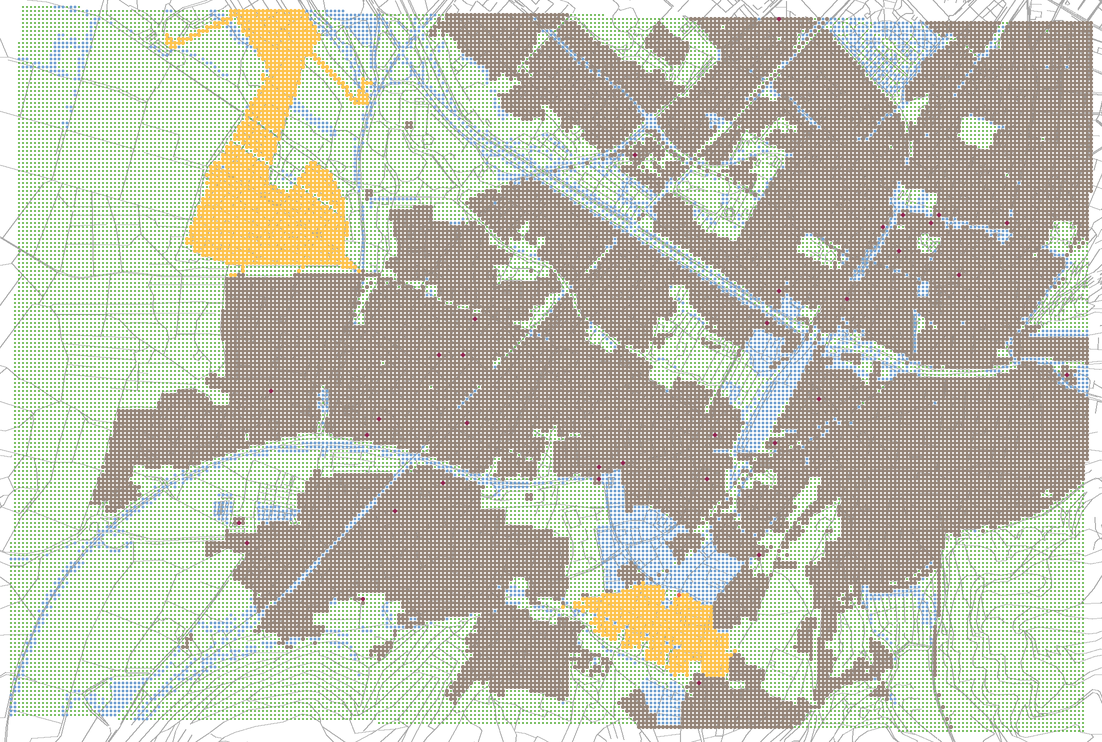
\includegraphics[width=0.48\textwidth]{figures/freiburg_validation_real.png}\hfill
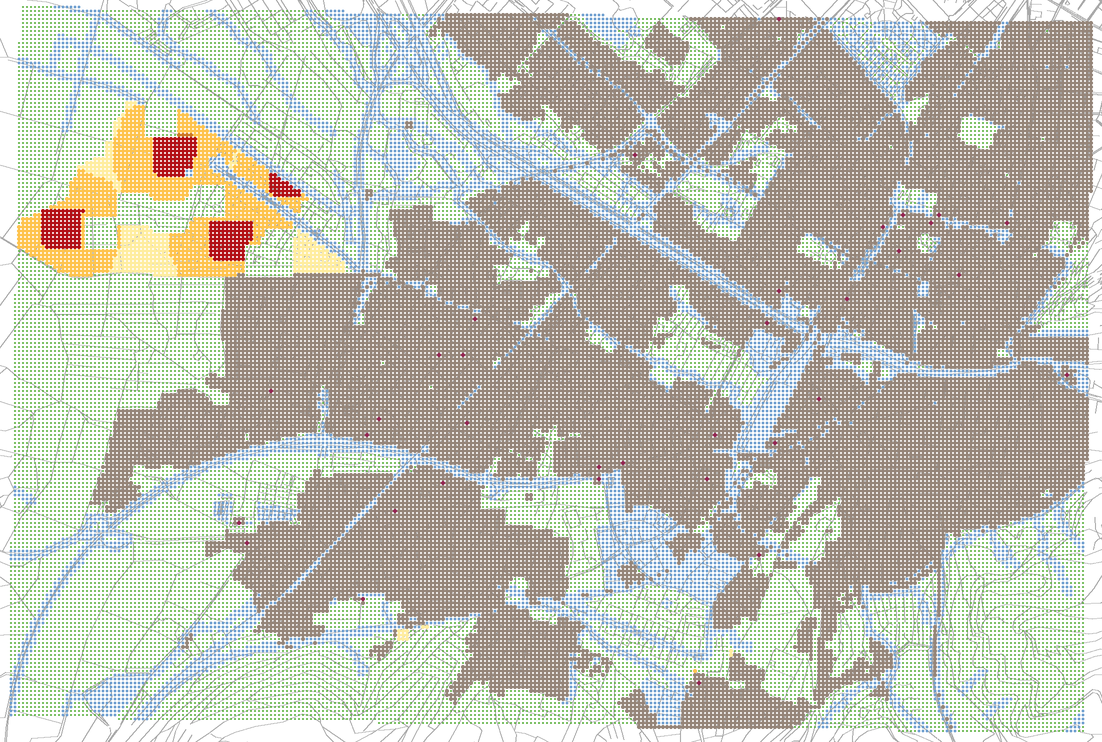
\includegraphics[width=0.48\textwidth]{figures/freiburg_validation_regrown_span200.png}\\[2pt]
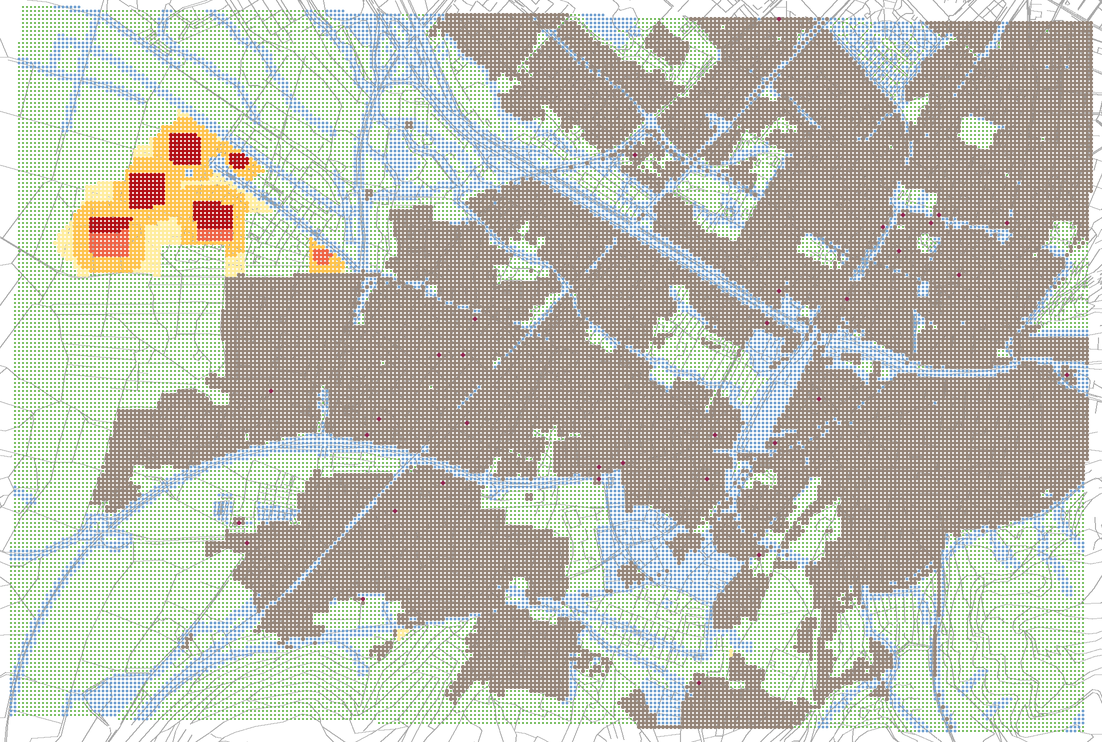
\includegraphics[width=0.48\textwidth]{figures/freiburg_validation_regrown.png}\hfill
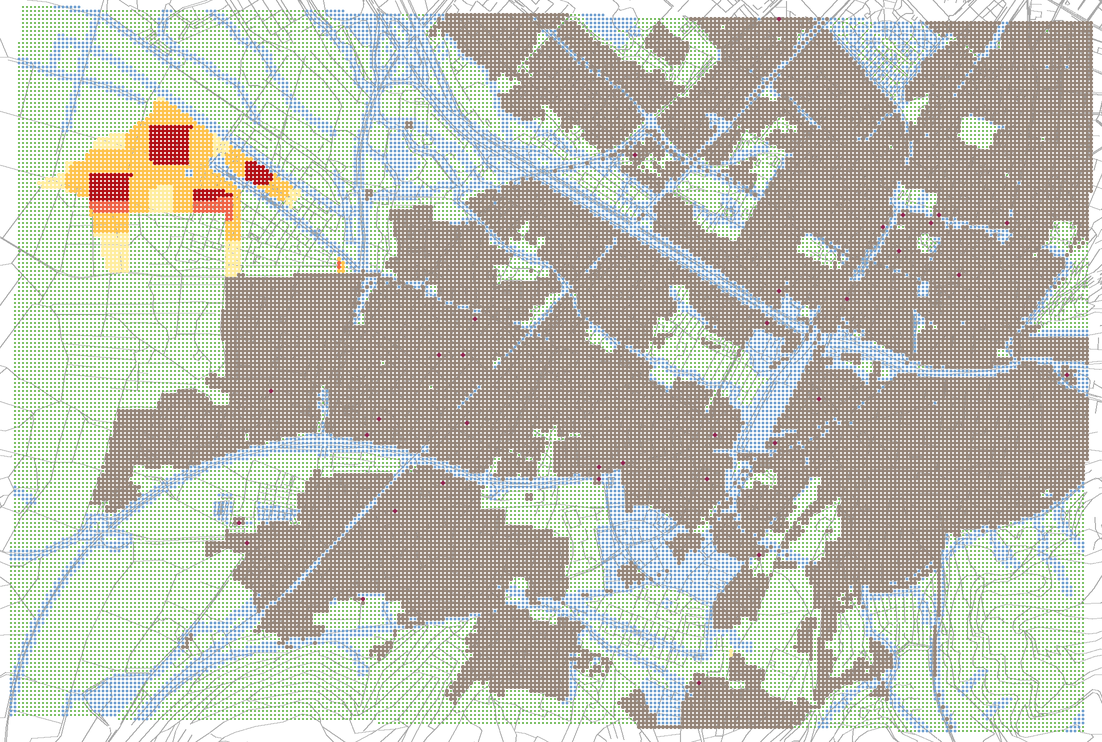
\includegraphics[width=0.48\textwidth]{figures/freiburg_validation_regrown_span600.png}
\caption{The Freiburg window as built (top left), with Rieselfeld and
Vauban as the development under assessment, and the regrown plan under
the pre-plan reading at minimum green spans of 200~m (top right), 400~m
(bottom left), and 600~m (bottom right). Regrown development falls
almost wholly inside the district boundaries (99\% at 200~m, 100\% at
400 and 600~m). Optimised placement, best of fifty runs, 25~m grid.}
\label{fig:freiburg}
\end{figure}

\section{Discussion}
\label{sec:discussion}

\subsection{Effects of the adaptations}

Real terrain changes what the walkability guarantee means. On the
abstract plain, the guarantee is a theorem about the rules; on real
inputs it becomes a property of a specific plan for a specific place,
which can be checked against the map. Results here do not compare
directly with published abstract-plain morphologies, because the walk
metric, the green rules, and the seeding guards all differ in the ways
Table~\ref{tab:rules} records.

The shared bounded grid walk for growth and scoring is the largest
departure. A street-network metric is common in walkability
analysis, and the implementation carried one for several releases before
we removed it for the reason given in Section~\ref{sec:gridprep}. The
bounded grid walk with carved barriers treats new and existing fabric on
the same terms while never crossing motorways, railways, and rivers.

\subsection{The post-processing gap}

The gap between the raw grown state and the plan options (84\% against 62\%
of target in the Cambourne demonstration window) is produced by pruning
alone. The pruned clusters are detached satellites that stayed below
the configured 1{,}000-person minimum when the run met its target, and
keeping them as free-standing settlements would overstate coverage. A
threshold that removes more than a quarter
of the grown population indicates that dispersal settings and the minimum
settlement size interact strongly, so the threshold warrants per-scenario
scrutiny in place of one universal default.

\subsection{Limitations}

Benefit is scored as a threshold, so 80~m and 780~m to a centre count the
same and coverage overstates the benefit of homes near the limit. A
distance-decay score would be more faithful to the isobenefit idea of
graded benefit. Any qualifying park serves its whole catchment regardless
of quality, which overstates green provision where park quality is poor.
Coverage counts every home in the window, so the metric does not compare
across windows with different shares of existing fabric, and
within-scenario comparisons are the intended reading. Every reported
figure comes from the best single run at one master seed and carries no
across-run spread, so we do not interpret small differences between
settings, such as footprint overlaps of 0.15 against 0.12 or mean walks a
few metres apart. The pipeline has
been exercised most heavily on Cambourne, and the Freiburg comparison is
a single case.

\section{Conclusion}
\label{sec:conclusion}

This implementation builds on the published model and turns Isobenefit
Urbanism into an instrument a planner can run on a real place. It
keeps the published growth rules recognisable and adapts them to real
geography through the departures that Table~\ref{tab:rules} records. The
plan-derivation pipeline
scores every run on walkable access, keeps the best single run, and
derives four outputs that run from the raw grown state through the
post-processed options to the three centre arrangements, with the walk
constraint enforced in every option. In three
case studies the same rules produce different answers where different
constraints dominate. The software, data, and parameters are public,
and the results rebuild from committed sources at fixed seeds.

The case studies here are hypothetical demonstrations, and a live
application would begin in dialogue with the residents and planners of
the place.

\subsection*{Acknowledgements}

This work is part of the Future Urban Growth project at the Bartlett School
of Planning, University College London. The authors thank the wider project
team: Luca D'Acci, Heeseo Rain Kwon, Stephen Marshall, and Valentina Marin
Maureira. The collection's guest editors, T.~Gabrieli (a co-author) and
L.~D'Acci (a member of the wider project team), are both connected to this
work; the submission is handled independently under the journal's
guest-editor policy.

\subsection*{Data availability}

All scenario inputs (boundaries, parameter presets, OpenStreetMap layers,
and slope bands) are committed in the project repository at
\url{https://github.com/UCL/BSP-isobenefit-qgis-plugin} under the
\texttt{scenarios/} directory. OpenStreetMap data \copyright{}
OpenStreetMap contributors, available under the Open Database License.
Slope layers derive from the Copernicus GLO-30 digital elevation model.

\subsection*{Code availability}

The simulation engine is published on PyPI as \texttt{isobenefit} and the
QGIS plugin through the official QGIS plugin repository; both are developed
in the repository above under the AGPL-3.0-or-later licence. The comparison
of Section~\ref{sec:freiburg} reruns with
\texttt{scripts/validate\_freiburg.py}: the default invocation gives the
pre-plan reading, \texttt{-{}-keep-green} the present-day reading, and
\texttt{-{}-min-green-span} 200 or 600 the span sweep.
\pending{archive a tagged release on Zenodo and cite the DOI here.}

\subsection*{Author contributions}

\pending{to be completed with the project team.}

\subsection*{Ethics declarations}

This article does not contain any studies with human participants or
animals performed by any of the authors, and informed consent is not
applicable.

\subsection*{Competing interests}

The authors declare no competing interests. L.~D'Acci, originator of
Isobenefit Urbanism and a guest editor of this collection, is a member of
the wider project team but not an author of this article; T.~Gabrieli is
also a guest editor of the collection and will take no part in its
editorial handling. \pending{confirm wording with the journal.}

\bibliographystyle{apalike}
\bibliography{refs}

\end{document}
